\documentclass{article}
\renewcommand{\familydefault}{\sfdefault}
\usepackage[a4paper, total={6in, 8in}]{geometry}
\usepackage{array}
\usepackage{amssymb}
\usepackage{mhchem}
\usepackage{chemarr}
\usepackage{graphicx}
\graphicspath{ {./images/} }

\title{Solutions}
\date{2021-04-20}
\author{Jeh}

\begin{document}
\maketitle
\pagenumbering{arabic}
   \section{One Mark Questions}
   \subsection{What is osmotic pressure?}
   The hydrostatic pressure (on the side of solution) that stops
   osmotic pressure of the solution.
   \begin{center} \textbf{OR} \end{center}
   The excess of pressure on the side of the solution that stops the
   net flow of solvent into solution through a semipermeable membrane
   is called as osmotic pressure.

   \subsection{A solution concentration is expressed in molarity and
   not in molality while considering osmotic pressure. Why?}
   \begin{enumerate}
	\item The osmotic pressure measurement are made at a specific
        constant temperature. Molarity remains constant at specific
	temperature. Molarity remains constant at specific
	temperature.
    	\item It is not necessary to express concentration in a
	temperature-independent unit like molality.
   \end{enumerate}
   Hence, the solute concentration is expressed in molarity while
   calculating osmotic pressure rather than molality while calculating
   osmotic pressure rather than molality.

   \subsection{Write the equation relating boiling point elevation to
   to the concentration of the solution.}
   The boiling point elevation is directly proportional to the molality
   of the solution. Thus,
   \begin{equation} \Delta T_b \propto m \end{equation}
   \begin{equation} T_b \propto K_b m \end{equation}
   where, m is the molality of solution. The proportionality constant
   $k_b$ is called boiling point elevation constant or molal elevation
   constant or ebuilioscopic constant.

   \subsection{What is van't Hoff factor?}
   van't Hoff factor (i) is defined as the ratio of colligative
   property of a solution of electrolyte divided by the colligative
   property of non electrolyte solution of the same concentration.\\
   Thus,
   \begin{equation}
   \frac{colligative property of electrolyte soltuion}
   {colligative property of non-electrolyte solution of the same
   solution of the same concentration}
   \end{equation}

   \begin{equation}
	   \frac{\Delta T_f}{(\Delta T_f)_0} = 
	   \frac{\Delta T_b}{(\Delta T_b )_0} = 
	   \frac{\Delta P} {(\Delta P)_0} =
	   \frac{\pi} {(\pi)_0}
   \end{equation}
   where the quantities without subscript refer to electrolytes and
   those with subscript to non electrolytes.

   \subsection{How is the van't Hoff factor related to degree of
   ionization?}
   The van't Hoff factor is related to degree of ionization as follows:
   \begin{equation} i = 1 + \alpha(n-1) \end{equation} or 
   \begin{equation} \alpha = \frac{i-1}{n-1} \end{equation}
   where, $\alpha$ = Degree of ionization/dissociation\\
   $i$ = van't Hoff factor\\
   $n$ = Moles of ions obtained from ionization of 1 mole of
   electrolyte.

   \subsection{Which of the following solution will have higher
   freezing point depression and why?\\
   i. 0.1m $NaCl$ \\
   ii. 0.05m $Al_2(SO_4)_3$} 
   For 0.1m $NaCl$:\\
   \ce{ $NaCl$ -> $Na^+$ + $Cl^-$ } \\
   $NaCl$ = 0.1m \ce{->} $Na^+$ = 0.1m + $Cl^-$ = 0.1m \\
   Total particles in solution = 0.2 mol \\\\
   For 0.05m $Al_2(SO_4)_3$ \\
   \ce{ $Al_2(SO_4)_3$ -> $2Al^3+$ + $3SO_4^2-$} \\
   For $Al_2(SO_4)_3$ = 0.05m \ce{->} $2Al$ = 0.1m + $3SO_4^2-$ = 0.15m
   \\Total particles in solution = 0.25 mol\\
   $Al_2(SO_4)_3$ solution contains more number of particles than $NaCl$
   solution. Hence, $Al_2(SO_4)_3$ solution has maximum $\Delta T_f$ \\
   Therefore, the freezing point depression of 0.05m $Al_2(SO_4)_3$ 
   solution will be higher than 0.1 m $NaCl$ solution.

   \subsection{State Raoult's law for a solution containing a
   nonvolatile solute}
   The Raoult's law states that, "the vapour pressure of solvent over
   the solution is equal to the vapour pressure of pure solvent
   multiplied by its mole fraction in the solution."

   \subsection{What is the effect on the boiling point of water if 1
   mole of methyl alcohol is added to $1dm^3$ of water? Why?}
   \begin{enumerate}
        \item When 1 mole of methyl alcohol is added to $1dm_3$ of
	water, the boiling point of water decreases.
	\item Methyl alcohol is a volatile liquid. Therefore, it
	increases the vapour pressure of a solution at given 
	temperature. Hence, the solution boils at lower temperature.
   \end{enumerate}

   \subsection{Which of the four colligative properties is most often
   used for molecular mass determination? Why?}
   \begin{enumerate}
	\item Among the four colligative properties, osmotic pressure
	is most often used for 	molecular mass determination.
	\item Osmotic pressure is much larger and therefore more 
	precisely measurable property than the colligative properties.
   \end{enumerate}

   \section{Two/Three Mark Questions}
   
   \subsection{How vapour pressure lowering is related to a rise in 
   the boiling point of solution}
   \begin{enumerate}
	\item At the boiling point of a liquid, its vapour pressure is
	equal to 1 atm.
	\item In order to reach boiling point, the solution and
	solvent must be heated to a temperature at which their 
	respective vapour pressures attain 1atm.
	\item At any given temperature the vapour pressure of a
	solution is lower than of pure solvent. Hence, the vapour
	pressure of solution needs a higher temperature to reach 1atm
	than that of needed for vapour pressure of solvent. 
   \end{enumerate}
   Therefore, vapour pressure lowering causes a rise in the boiling 
   point of a solution.

   \subsection{What are isotonic and hypertonic solutions?}
   i. \textbf{Isotonic Solutions} \\\\
   Two or more solutions having the same osmotic pressure are said to
   be isotonic solutions.\\
   e.g For example, 0.1M urea solution and 0.1M sucrose soltuion are
   isotonic because their osmotic pressure are equal. Such solutions
   have the same molar concentrations but different concentrations in
   g/L. If these solutions are seperated by a semipermeable membrane,
   there is no flow of solvent in either direction. \\
   ii. \textbf{Hyprtonic Solution} \\\\
   If two solutions have unequal osmotic pressure, the more
   concentrated solution with higher osmotic pressure is said to be
   the hypertonic solution.\\
   e.g For example, if osmotic pressure of sucrose solution is higher
   that of urea solution, the sucrose solution is hypertonic to urea
   solution.

   \subsection{A solvent and its solvent containing a nonvolatile
   solute are seperated by a semipermeable membrane. Does the flow of
   solvent occur in both directions? Comment giving a reason.}
   \begin{enumerate}
	\item When a solution and pure solvent or two solutions of
	different concentrations are seperated by a semipermeable
	membrane, the solvent molecules pass through the membrane.
	\item The passage of solvent molecules through the 
	semipermeable membrane takes place in both direction, since
	the solvent is on both sides of membrane.
	\item However, the rate of passage of solvent molecules into
	solution or from a more dilute solution to more concentrated
	solution is found to be greater than the rate in reverse 
	direction.
	\item This is favorable since the vapour pressure of solvent
	is greater than that of solution.
   \end{enumerate}

   \subsection{Explain reverse osmosis.}
   \begin{enumerate}
	\item If a pressure is larger than the osmotic pressure is
	applied to the soltuion side, then pure solvent from the
	solution passes into pure solvent side through the
	semipermeable membrane. This phenomenon is called reverse
	osmosis.
	\item For example, consider fresh water and salt water 
	seperated by a semipermeable membrane. When the pressure
	larger than the osmotic pressure of solution is applied to
	the solution, pure water from salty water passes into fresh
	water through the membrane. Thus, the direction of osmosis
	can be reversed by applying a pressure larger than the osmotic
	pressure.
	\item The schematic set up for reverse osmosis is as follows:
   \end{enumerate}
   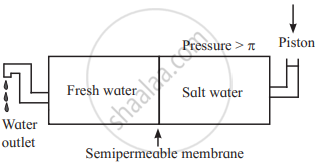
\includegraphics[scale=0.5]{reverse}

   \subsection{How molar mass of solute is determined by osmotic
   pressure measurement?}
   \begin{enumerate}
	\item For very dilute solutions, the osmotic pressure follows
	the equation, 
	\begin{equation} \pi = \frac{n_2RT}{V} \end{equation}
	\item If the mass of solute in V litres of solution is W2 and
	its molar mass is 
	\begin{equation} M_2, then n_2 = \frac{W_2}{M_2} \end{equation}
   \end{enumerate}
   Substituting the value of $n_2$ in equation (1), we get
   \begin{equation} \pi = \frac{W_2RT}{M_2V} \end{equation}
   \begin{equation} \therefore M_2 = \frac{W_2RT}{\pi V} \end{equation}
   This formula can be used for the calcuation of molar mass of
   nonionic solute (i.e nonelectrolytes) by osmotic pressure 
   measurement.

   \subsection{Why vapour pressure of a solvent is lowered by
   dissolving a nonvolatile solute into it?}
   \begin{enumerate}
	\item Vapour pressure of a liquid depends on the ease with
	which the molecules escape from the surface of liquid.
	\item When a nonvolatile solute is dissolved in a solvent,
	some of the surface molecules of the solvent are replaced
	by nonvolatile solute molecules. These solute molecules do not
	contribute to vapour above the solution.
	\item Thus, the number of solvent molecules available for
	vapourization per unit surface of the pure solvent.
	\item As a result the solvent molecules at the surface of
	solution vapourize at a slower rate than pure solvent. This
	results in lowering of vapou pressure.
   \end{enumerate}

   \subsection{Using Raoult's law, how wil you show that $P_1^0x_2$
   ? Where, $x_2$ is the mole fraction of solute in the solution and
   $P_1^0$ vapour pressure of pure solvent.}
   \begin{enumerate}
	\item Raoult's law expresses the quantitative relationship
	between vapour pressure of solution and vapour pressure of
	the solvent.
	\item In soltuions of nonvolatile solutes, the law is
	applicable only to the volatile solvent.
	\item The law states that, "the vapour pressure of solvent
	over the solution is equal to vapour pressure of pure solvent.
	\item The law states that, "the vapour pressure of solvent
	over the solution is equal to the vapour pressure of pure
	solvent multiplied by its mole fraction in the solution."
	\item Suppose that for a binary solution containing solvent
	and one nonelectrolytes solute, $P_1$ is the vapour pressure
	of solvent over the solution, $x_1$ and $x_2$ are the mole
	fractions of solvent and solute, respectively and $P_1^0$
	is the vapour pressure of pure solvent, then $P_1 = P_1^0x_1$
	\item Since, $x_1 = 1 - x_2$,
	\begin{equation} P_1 = P_1^0x_1 = P_1^0(1-x_2) = 
	P_1^0 - P_1^0x_2 \end{equation}
	\begin{equation}\therefore P_1^0 - P_1 = P_1^0x_2
	\end {equation}
	\begin{equation} \therefore \Delta P = P_1^0x_2 
	(\because \Delta P is the lowering of vapour pressure)
	\end{equation}
	Note : A plot of $P_1$ versus $x_1$ is a straight as shown
	below.\\
	\textbf{Variation of vapour pressure of solution with mole
	fraction of solvent}\\
	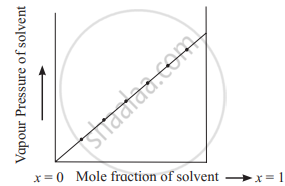
\includegraphics[scale=0.5]{vapour}
   \end{enumerate}

   \subsection{While considering boiling point elevation and freezing
   point of depression a solution concentration is expressed in 
   molality and not in molarity. Why?}
   \begin{enumerate}
	\item In boiling point elevation and freezing point depression,
	we deal with the systems whose temperature is not constant.
	\item We cannot express the concentration of the solution in
	molarity becaues it changes temperature but whereas molality
	is temperature independent.
   \end{enumerate}
   Hence, while considering boiling point elevation and freezing point
   depression a solution concentration is expressed in molality and
   not in molarity.

   \subsection{Derive the relationship between the degree of
   dissociation of an electrolyte and van't Hoff factor.}
   \begin{enumerate}
	\item The weak electrolytes involves the concept of degree 
	of dissociation $(\alpha)$ that changes the van't Hoff factor.
	\item Consider an electrolyte $A_xB_y$ that dissociates in
	aqueous solution as 
	\begin{center}
	\begin{tabular}{ | m{20em} | m{20em} | }
	\hline
	\vspace{4em} &  $A_xB_y$ $\rightleftharpoons$ $xA^{y+}$ + 
	$yB^{x-}$ \\
	\hline
	Initially & 1mol \hspace{0.7cm} 0 \hspace{0.7cm} 0 \\
	\hline
	At equilibrium & (1 - $\alpha$)mol \hspace{0.7cm} 
	(x $\alpha$ mol)
	\hspace{0.7cm} (y $\alpha$ mol) \\
	\hline
	\end{tabular}
	\end{center}
	\item If $\alpha$ is the degree of dissociation of electrolyte,
	then the moles of cations are $x\alpha$ and those of anions 
	are $y\alpha$ equilibrium. We have dissolved just 1 mol of 
	electrolyte dissociates and $(1 - \alpha)$ mol remains 
	undisssociated at equilibrium.\\
	Total moles after dissociation = 
	\begin{equation}
		(1 - \alpha) + (x\alpha) + (y\alpha)
	\end{equation}
	\begin{equation}
		= 1 + \alpha(x + y -1)
	\end{equation}
	\begin{equation}
		= 1 + \alpha(n-1) \\
	\end{equation}
	Where, $n = x + y =$ moles of ions obtained from dissociation
	of 1 mole of electrolyte.
	\item The van't Hoff factor gives as
	\begin{equation}
		i = \frac{actual moles of particles insolution after
		dissociation}{moles of formula units dissolved in
		solution}
	\end{equation}
	\begin{equation}
		= \frac{1 + \alpha(n-1)}{1}
	\end{equation}
	Hence, $i = 1 + \alpha(n-1)$ or $\alpha = \frac{i + 1} {n - 1}$
   \end{enumerate}
   \subsection{What is the effect of temperature on solubility of
   solids in water? Give examples.}
   \begin{enumerate}
	\item The effect of temperature on solubility of a substance
	depends on enthalpy of solution.
	\begin{enumerate}
	    \item When the substance dissolves in water by an 
	    endothermic process, that is, with the absorption of heat,
	    its adsorption of heat, its solubility increases with an
	    increase in temperature.\\
	    e.g KCl dissolves in water by endothermic process.
    	    \item On the other hand, when the substance dissolves in
	    water by an exothermic process, that is, with the release
	    of heat, its solubility decreases with an increase in 
	    temperature.\\
	    e.g $CaCl_2$ and $Li_2SO_4.H_2O$ dissolves in water
	    releasing heat.
	\end{enumerate}
	\item It is important to understand that there is no direct 
	correlation between solubility and exothermicity or 
	endothermicity. For example, dissolution of $CaCl_2$ in water
	is exothermic and that of $NH_4NO_3$ is endothermic. However,
	the solubility of these substances increases with the
	temperature.
   \end{enumerate}
   \subsection{Explain with diagram that boiling point elevation 
   in terms of vapour pressure lowering.}
   \begin{enumerate}
	\item The vapour pressure of a solution and pure solvent are
	plotted as a function of temperature in the given diagram.
	\item At any temperature, the vapour pressure of solution is
	lower than that of pure solvent. Hence, the vapour pressure-
	temperature curve of solution (CD) lies below that of solvent
	(AB)
	\item The difference between two vapour pressure increases
	as temperature and vapour pressure increases as predicted by
	the following equation,
	\begin{equation} \Delta P = P_1^0 X_2 \end{equation}
	\item The intersection of curve CD with line corresponding to
	760mm is the boiling point solution. The similar intersection
	of the curve AB is the boiling point of pure solvent. It is
	clear from the diagram that the boiling point solution $(T_b)$
	is higher than that of pure solvent $(T_b^0)$
	\item At the boiling point of liquid its vapour pressure is
	equal to 1atm.
	\item In order to reach the boiling point, the solution and 
	solvent must be heated to a temperature at which their
	respective vapour pressure attain 1atm.
	\item At any given temperature the vapour pressure of solution
	is lower than that of pure solvent. Hence, the vapour pressure
	of solution needs a higher temperature to reach 1atm than that
	for vapour pressure of solvent.
	\item In other words, the solution must be heated to higher
	temperature to cause it to boil than pure solvent.
   \end{enumerate}
   \begin{center}
	   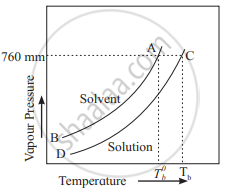
\includegraphics[scale=0.7]{prestemp}
   \end{center}
   	
\end{document}
